\documentclass[12pt,a4paper]{article}
\usepackage{lmodern}

\usepackage{enumitem}
\usepackage{placeins}
\usepackage{amssymb,amsmath}
\usepackage{ifxetex,ifluatex}
\usepackage{fixltx2e} % provides \textsubscript
\ifnum 0\ifxetex 1\fi\ifluatex 1\fi=0 % if pdftex
  \usepackage[T1]{fontenc}
  \usepackage[utf8]{inputenc}
\else % if luatex or xelatex
  \ifxetex
    \usepackage{mathspec}
    \usepackage{xltxtra,xunicode}
  \else
    \usepackage{fontspec}
  \fi
  \defaultfontfeatures{Mapping=tex-text,Scale=MatchLowercase}
  \newcommand{\euro}{€}
\fi
% use upquote if available, for straight quotes in verbatim environments
\IfFileExists{upquote.sty}{\usepackage{upquote}}{}
% use microtype if available
\IfFileExists{microtype.sty}{%
\usepackage{microtype}
\UseMicrotypeSet[protrusion]{basicmath} % disable protrusion for tt fonts
}{}
\usepackage[lmargin = 2cm, rmargin = 2cm, tmargin = 2cm, bmargin = 2.5cm]{geometry}


% Figure Placement:
\usepackage{float}
\let\origfigure\figure
\let\endorigfigure\endfigure
\renewenvironment{figure}[1][2] {
    \expandafter\origfigure\expandafter[H]
} {
    \endorigfigure
}

%%%% Jens %%%%
\usepackage{titlesec}
\DeclareMathOperator*{\argmax}{arg\,max}
\DeclareMathOperator*{\argmin}{arg\,min}
\renewcommand{\vec}{\operatorname{vec}}
\newcommand{\tr}{\operatorname{tr}}
\newcommand{\Var}{\operatorname{Var}} % Variance
\newcommand{\MSE}{\operatorname{MSE}} % Variance
\newcommand{\VAR}{\operatorname{VAR}} % Vector autoregression
\newcommand{\Lag}{\operatorname{L}} % Lag operator
\newcommand{\Cov}{\operatorname{Cov}}
\newcommand{\diag}{\operatorname{diag}}
\newcommand{\adj}{\operatorname{adj}}
\newcommand{\loglik}{\operatorname{ll}}

\usepackage{centernot}

\allowdisplaybreaks

\titleformat{\section}
{\normalfont\large\bfseries}{\thesection}{1em}{}

\newcommand{\tmpsection}[1]{}
\let\tmpsection=\section
\renewcommand{\section}[1]{\tmpsection{\underline{#1}} }





%% citation setup
\usepackage{csquotes}

\usepackage[backend=biber, maxbibnames = 99, style = apa]{biblatex}
\setlength\bibitemsep{1.5\itemsep}
\addbibresource{R_packages.bib}
\usepackage{color}
\usepackage{fancyvrb}
\newcommand{\VerbBar}{|}
\newcommand{\VERB}{\Verb[commandchars=\\\{\}]}
\DefineVerbatimEnvironment{Highlighting}{Verbatim}{commandchars=\\\{\}}
% Add ',fontsize=\small' for more characters per line
\usepackage{framed}
\definecolor{shadecolor}{RGB}{248,248,248}
\newenvironment{Shaded}{\begin{snugshade}}{\end{snugshade}}
\newcommand{\AlertTok}[1]{\textcolor[rgb]{0.94,0.16,0.16}{#1}}
\newcommand{\AnnotationTok}[1]{\textcolor[rgb]{0.56,0.35,0.01}{\textbf{\textit{#1}}}}
\newcommand{\AttributeTok}[1]{\textcolor[rgb]{0.77,0.63,0.00}{#1}}
\newcommand{\BaseNTok}[1]{\textcolor[rgb]{0.00,0.00,0.81}{#1}}
\newcommand{\BuiltInTok}[1]{#1}
\newcommand{\CharTok}[1]{\textcolor[rgb]{0.31,0.60,0.02}{#1}}
\newcommand{\CommentTok}[1]{\textcolor[rgb]{0.56,0.35,0.01}{\textit{#1}}}
\newcommand{\CommentVarTok}[1]{\textcolor[rgb]{0.56,0.35,0.01}{\textbf{\textit{#1}}}}
\newcommand{\ConstantTok}[1]{\textcolor[rgb]{0.00,0.00,0.00}{#1}}
\newcommand{\ControlFlowTok}[1]{\textcolor[rgb]{0.13,0.29,0.53}{\textbf{#1}}}
\newcommand{\DataTypeTok}[1]{\textcolor[rgb]{0.13,0.29,0.53}{#1}}
\newcommand{\DecValTok}[1]{\textcolor[rgb]{0.00,0.00,0.81}{#1}}
\newcommand{\DocumentationTok}[1]{\textcolor[rgb]{0.56,0.35,0.01}{\textbf{\textit{#1}}}}
\newcommand{\ErrorTok}[1]{\textcolor[rgb]{0.64,0.00,0.00}{\textbf{#1}}}
\newcommand{\ExtensionTok}[1]{#1}
\newcommand{\FloatTok}[1]{\textcolor[rgb]{0.00,0.00,0.81}{#1}}
\newcommand{\FunctionTok}[1]{\textcolor[rgb]{0.00,0.00,0.00}{#1}}
\newcommand{\ImportTok}[1]{#1}
\newcommand{\InformationTok}[1]{\textcolor[rgb]{0.56,0.35,0.01}{\textbf{\textit{#1}}}}
\newcommand{\KeywordTok}[1]{\textcolor[rgb]{0.13,0.29,0.53}{\textbf{#1}}}
\newcommand{\NormalTok}[1]{#1}
\newcommand{\OperatorTok}[1]{\textcolor[rgb]{0.81,0.36,0.00}{\textbf{#1}}}
\newcommand{\OtherTok}[1]{\textcolor[rgb]{0.56,0.35,0.01}{#1}}
\newcommand{\PreprocessorTok}[1]{\textcolor[rgb]{0.56,0.35,0.01}{\textit{#1}}}
\newcommand{\RegionMarkerTok}[1]{#1}
\newcommand{\SpecialCharTok}[1]{\textcolor[rgb]{0.00,0.00,0.00}{#1}}
\newcommand{\SpecialStringTok}[1]{\textcolor[rgb]{0.31,0.60,0.02}{#1}}
\newcommand{\StringTok}[1]{\textcolor[rgb]{0.31,0.60,0.02}{#1}}
\newcommand{\VariableTok}[1]{\textcolor[rgb]{0.00,0.00,0.00}{#1}}
\newcommand{\VerbatimStringTok}[1]{\textcolor[rgb]{0.31,0.60,0.02}{#1}}
\newcommand{\WarningTok}[1]{\textcolor[rgb]{0.56,0.35,0.01}{\textbf{\textit{#1}}}}
\usepackage{graphicx}
\makeatletter
\def\maxwidth{\ifdim\Gin@nat@width>\linewidth\linewidth\else\Gin@nat@width\fi}
\def\maxheight{\ifdim\Gin@nat@height>\textheight\textheight\else\Gin@nat@height\fi}
\makeatother
% Scale images if necessary, so that they will not overflow the page
% margins by default, and it is still possible to overwrite the defaults
% using explicit options in \includegraphics[width, height, ...]{}
\setkeys{Gin}{width=\maxwidth,height=\maxheight,keepaspectratio}
\ifxetex
  \usepackage[setpagesize=false, % page size defined by xetex
              unicode=false, % unicode breaks when used with xetex
              xetex]{hyperref}
\else
  \usepackage[unicode=true, linktocpage = TRUE]{hyperref}
\fi
\hypersetup{breaklinks=true,
            bookmarks=true,
            pdfauthor={Dr.~Yannick Hoga},
            pdftitle={Multivariate Time Series Analysis},
            colorlinks=true,
            citecolor=black,
            urlcolor=black,
            linkcolor=black,
            pdfborder={0 0 0}}
\urlstyle{same}  % don't use monospace font for urls
\setlength{\parindent}{0pt}
\setlength{\parskip}{6pt plus 2pt minus 1pt}
\setlength{\emergencystretch}{3em}  % prevent overfull lines
\setcounter{secnumdepth}{5}

%%% Use protect on footnotes to avoid problems with footnotes in titles
\let\rmarkdownfootnote\footnote%
\def\footnote{\protect\rmarkdownfootnote}

%%% Change title format to be more compact
\usepackage{titling}

% Create subtitle command for use in maketitle
\newcommand{\subtitle}[1]{
  \posttitle{
    \begin{center}\large#1\end{center}
    }
}

\setlength{\droptitle}{-2em}
  \title{Multivariate Time Series Analysis}
  \pretitle{\vspace{\droptitle}\centering\huge}
  \posttitle{\par}
\subtitle{Solution Exercise Sheet 6}
  \author{Dr.~Yannick Hoga}
  \preauthor{\centering\large\emph}
  \postauthor{\par}
  \date{}
  \predate{}\postdate{}


%% linespread settings

\usepackage{setspace}

\onehalfspacing


% Language Setup

\usepackage{ifthen}
\usepackage{iflang}
\usepackage[super]{nth}
\usepackage[ngerman, english]{babel}

%Acronyms
\usepackage[printonlyused, withpage, nohyperlinks]{acronym}
\usepackage{changepage}

% Multicols for the Title page
\usepackage{multicol}


% foot


\begin{document}

\selectlanguage{english}

%%%%%%%%%%%%%% Jens %%%%%
\numberwithin{equation}{section}




\restoregeometry


%%% Header 

\begin{minipage}{0.6\textwidth}
University of Duisburg-Essen\\
Faculty of Business Administration and Economics\\
Chair of Econometrics\\
\end{minipage}

%\begin{minipage}{0.4\textwidth}
	\begin{flushright}
	\vspace{-3cm}
	\includegraphics*[width=5cm]{../Includes/duelogo_en.png}\\
	\vspace{.125cm}
	\end{flushright}
%\end{minipage}
%\vspace{.125cm}
\hspace{-0.005cm}Winter Term 2019/2020

\vspace{0.05cm}

\begin{center}
	\vspace{.25cm}
	Dr.~Yannick Hoga \hspace{.5cm} Thilo Reinschlüssel \\
	\vspace{.25cm}
	\textbf{\Large{Multivariate Time Series Analysis}}\\
	\vspace{.25cm}
	\textbf{\large{Solution Exercise Sheet 6}}\\
	\vspace{.125cm}
\end{center}




% body from markdown

\hypertarget{exercise-1-model-selection---review}{%
\section{Exercise 1: Model Selection -
Review}\label{exercise-1-model-selection---review}}

\begin{itemize}
  \item[a)] Is the MSE scale-invariant? 
\end{itemize}

\emph{Solution:}

No, the MSE is scale-dependent. Take the following \(\VAR(1)\) as an
example (\(\mu_z = 0 \ \text{w.l.o.g}\)):

\begin{align*}
z_t =  \phi_1 z_{t-1} + a_t\\
\end{align*}

Define \(k_t := b z_t\) where \(b\) is a scalar.

\begin{align*}
  \Rightarrow k_t & = b z_t = \phi_1 b z_{t-1} + e_t \\
  \Leftrightarrow e_T & = k_t - \phi_1 k_t = b \cdot \left(z_t - \phi z_{t-1} \right) = b \cdot a_t\\
  \\
  \MSE(\hat{k}_{t, t+1} ) & = \mathbb{E} \left[ e_{t+1}^{2}\right] = \mathbb{E} \left[ (b a_{t+1})^{2}\right] \\
   & = b^2 \cdot \mathbb{E} \left( a_{t+1}^{2}\right)\\
   & = b^2 \cdot  \MSE(\hat{z}_{t, t+1} )\\
\end{align*}

where \(\hat{k}_{t, t-1}, \hat{z}_{t, t-1}\) are the \(\VAR (1)\)
predictions.

\begin{itemize}
  \item[b)] What is the fundamental trade-off which information criteria are supposed to balance? 
\end{itemize}

\emph{Solution:}

\begin{align*}
  IC (l) & = \underbrace{\log \left( A \right)}_{\substack{\text{Fit} \\ \\  \sim \ \log(|\MSE|)}} + \underbrace{\dfrac{l}{T} \ c_T}_{\text{complexity}}
\end{align*}

\begin{itemize}
  \item[c)] Does a linear transformation affect the value of the information criteria? Does it also influence the location of the minima?  
\end{itemize}

\emph{Solution:}

Again, the \(\VAR(1)\) example.
\[z_t = \phi_0 + \phi_1 z_{t-1} +a_t \quad \mid z_t \ \text{is} \ k \times 1 \]

Linear transformation: \(k_t = B z_t + c\)

\begin{itemize}
  \item[$\Rightarrow$] $c$ is covered by $\phi_0 = \phi_0 + c$, no problem. w.l.o.g. we omit that part.
  \item[$\Rightarrow$] $\underbrace{B z_t}_{=: k_t} = \phi_1 \underbrace{B z_{t-1}}_{=: k_{t-1}} + \underbrace{B a_t}_{=: e_t}$
\end{itemize}

\begin{align*}
  \Rightarrow \left| \MSE \left(\hat{k}_{t, t+1} \right) \right| & = \left| \mathbb{E} \left(e_t e_t^{'} \right) \right| \\
  & = \left| \mathbb{E} \left(\underbrace{B}_{k \times k} \underbrace{a_t a_t^{'}}_{k \times k} \underbrace{B^{'}}_{k \times k}\right) \right|\\
  & = \left| B \ \mathbb{E} \left( \underbrace{a_t a_t^{'} }_{= \MSE (\hat{z}_{t, t+1})}\right) \ B \right|\\
  & = \left| B \right| \ \left| \MSE \left( \hat{z}_{t, t+1}) \right) \right| \ \left| B \right| \\
  & = \left(\left| B \right|\right)^2 \ \left| \MSE \left( \hat{z}_{t, t+1}) \right) \right| 
\end{align*}

\(\Rightarrow\) The linear transformation affects the value of the ICs.
But as long as \(|B| \neq 0\) (non-singular), the
\(\MSE\left( \hat{k}_{t,t+1} \right)\) is minimal where
\(\MSE\left( \hat{z}_{t,t+1} \right)\) has its minimum.

Example for singular \(B\):

\[B = \begin{pmatrix} 1 & 1 \\ 1 & 1 \end{pmatrix}, \begin{pmatrix} 1 & 0 \\ 0 & 0 \end{pmatrix}, \begin{pmatrix} 1 & 0 & 0 \\ 0 & 0 & 0 \\ 0 & 0 & 1 \end{pmatrix}\]

\begin{itemize}
  \item[d)] Finally: Are OLS standard errors scale invariant? 
\end{itemize}

\emph{Solution:}

In (3-3, lecture slides), we write the \(\VAR(p)\) model as:
\(Z = X\beta + A\)

\begin{align*}
  \Leftrightarrow A & = Z - X \beta \\
  \text{and} \;\hat{\beta} & = \left( X^{'} X\right)^{-1} X^{'} Z = \beta + \left( X^{'} X\right)^{-1} X^{'} A \\
  \\
  \Leftrightarrow  \Var \left( \hat{\beta} - \beta \right) & = \mathbb{E} \left( \left(X^{'} X \right)^{-1}  X^{'} A \left[ (X^{'} X)^{-1} X^{'} A \right]^{'} \right) \\
  & = \mathbb{E} \left( \left(X^{'} X \right)^{-1}  X^{'} A  A^{'} X \left(X^{'} X \right)^{-1} \right)
\end{align*}

If we scale \(Z\) by the scalar \(b\), we also scale
\(X = \left(LZ, L^2 Z, \ldots \right)\) and \(A\) by \(b\).
\(\Rightarrow \tilde{X} = bX, \tilde{Z} = bZ, \tilde{A} = bA, \tilde{\beta} = \dfrac{b^2}{b^2} \beta\).

\begin{align*}
  \Leftrightarrow \Var \left( \hat{\tilde{\beta}} - \beta \right) & = \mathbb{E} \left(\left(\tilde{X}^{'} \tilde{X} \right)^{-1} \tilde{X}^{'} \tilde{A} \tilde{A}^{'} \tilde{X} \left(\tilde{X}^{'} \tilde{X} \right)^{-1} \right)\\
   & = \mathbb{E} \left( \dfrac{1}{b^2} \left(\tilde{X}^{'} \tilde{X} \right)^{-1} b^2 \tilde{X}^{'} \tilde{A} \tilde{A}^{'} \tilde{X} b^2  \dfrac{1}{b^2}\left(\tilde{X}^{'} \tilde{X} \right)^{-1} \right) \\
   & = \left( \hat{\beta} - \beta \right)
\end{align*}

\(\Rightarrow\) Standard errors are scale-invariant! (similar to
\(R^2\))

\hypertarget{exercise-2-simplicfication-and-forecasting---macroeconomic-data}{%
\section{Exercise 2: Simplicfication and Forecasting - Macroeconomic
Data}\label{exercise-2-simplicfication-and-forecasting---macroeconomic-data}}

Reconsider Exercise 2 from Exercise Sheet 5. Again, please import/load
the dataset \texttt{us\_macrodata.Rda} into your workspace and compute
the growth rates of the variables appearing non-stationary. There are
still 5 variables---CPI, Real GDP, the unemployment rate, general
private investment and the debt-to-GDP ratio. All series have been
sampled quarterly and were seasonally adjusted before downloaded from
\emph{FRED}.

\begin{itemize}
  \item[a)] Fit a $\VAR(p)$ model according to the Hannan-Quinn information-criteria? 
\end{itemize}

\emph{Solution:}

\begin{Shaded}
\begin{Highlighting}[]
\CommentTok{# loading the Data}
\KeywordTok{load}\NormalTok{(}\DataTypeTok{file =}\NormalTok{ here}\OperatorTok{::}\KeywordTok{here}\NormalTok{(}\StringTok{"exercise_MTSA/00_data/us_macrodata.Rda"}\NormalTok{))}

\CommentTok{# compute growth rates (diff-logs) of every variable except unemployment}
\NormalTok{macdata <-}\StringTok{ }\KeywordTok{cbind}\NormalTok{(}\KeywordTok{diff}\NormalTok{(}\KeywordTok{log}\NormalTok{(us.macro_series}\OperatorTok{$}\NormalTok{cpi)),}
                 \KeywordTok{diff}\NormalTok{(}\KeywordTok{log}\NormalTok{(us.macro_series}\OperatorTok{$}\NormalTok{rgdp)),}
\NormalTok{                 us.macro_series}\OperatorTok{$}\NormalTok{unemprate[}\OperatorTok{-}\KeywordTok{nrow}\NormalTok{(us.macro_series)],}
                 \KeywordTok{diff}\NormalTok{(}\KeywordTok{log}\NormalTok{(us.macro_series}\OperatorTok{$}\NormalTok{gp_investment)),}
                 \KeywordTok{diff}\NormalTok{(}\KeywordTok{log}\NormalTok{(us.macro_series}\OperatorTok{$}\NormalTok{debt_gdp)))}
\end{Highlighting}
\end{Shaded}

\begin{Shaded}
\begin{Highlighting}[]
\KeywordTok{VARorder}\NormalTok{(}\DataTypeTok{x =}\NormalTok{ macdata, }\DataTypeTok{maxp =} \DecValTok{25}\NormalTok{)}
\end{Highlighting}
\end{Shaded}

\begin{verbatim}
## selected order: aic =  25 
## selected order: bic =  1 
## selected order: hq =  3 
## Summary table:  
##        p      AIC      BIC       HQ     M(p) p-value
##  [1,]  0 -35.2115 -35.2115 -35.2115   0.0000  0.0000
##  [2,]  1 -40.4514 -40.0347 -40.2827 909.1993  0.0000
##  [3,]  2 -40.8183 -39.9850 -40.4809  99.6246  0.0000
##  [4,]  3 -41.0619 -39.8120 -40.5559  77.3593  0.0000
##  [5,]  4 -41.2039 -39.5373 -40.5293  59.5643  0.0001
##  [6,]  5 -41.2134 -39.1301 -40.3701  38.3056  0.0432
##  [7,]  6 -41.0723 -38.5724 -40.0603  15.8407  0.9195
##  [8,]  7 -41.0958 -38.1792 -39.9151  37.5698  0.0509
##  [9,]  8 -41.1136 -37.7804 -39.7643  35.4524  0.0803
## [10,]  9 -41.0453 -37.2955 -39.5274  23.2832  0.5610
## [11,] 10 -41.0395 -36.8730 -39.3529  29.8782  0.2289
## [12,] 11 -41.1118 -36.5287 -39.2565  37.6673  0.0498
## [13,] 12 -41.2495 -36.2497 -39.2255  43.2609  0.0131
## [14,] 13 -41.2170 -35.8005 -39.0243  23.3435  0.5575
## [15,] 14 -41.3543 -35.5212 -38.9930  39.3061  0.0343
## [16,] 15 -41.3199 -35.0701 -38.7899  20.9530  0.6952
## [17,] 16 -41.3009 -34.6345 -38.6023  21.2580  0.6781
## [18,] 17 -41.4345 -34.3515 -38.5672  33.1211  0.1281
## [19,] 18 -41.4278 -33.9281 -38.3918  19.8881  0.7527
## [20,] 19 -41.4337 -33.5174 -38.2291  19.6110  0.7669
## [21,] 20 -41.5126 -33.1796 -38.1393  23.4546  0.5510
## [22,] 21 -41.7971 -33.0475 -38.2552  35.2611  0.0836
## [23,] 22 -42.2191 -33.0528 -38.5085  40.8826  0.0236
## [24,] 23 -42.5442 -32.9612 -38.6649  32.1296  0.1543
## [25,] 24 -42.7201 -32.7205 -38.6722  21.7025  0.6529
## [26,] 25 -43.1356 -32.7193 -38.9190  30.4528  0.2078
\end{verbatim}

The Hannan-Quinn information criteria suggests to fit a \(\VAR(3)\).

\begin{Shaded}
\begin{Highlighting}[]
\NormalTok{var_}\FloatTok{3.}\NormalTok{fit <-}\StringTok{ }\KeywordTok{VAR}\NormalTok{(}\DataTypeTok{x =}\NormalTok{ macdata, }\DataTypeTok{p =} \DecValTok{3}\NormalTok{, }\DataTypeTok{include.mean =} \OtherTok{TRUE}\NormalTok{)}
\end{Highlighting}
\end{Shaded}

\begin{verbatim}
## Constant term: 
## Estimates:  -0.001113295 -0.00410686 0.3701935 -0.06283592 -0.004091712 
## Std.Error:  0.002102026 0.003129741 0.08098804 0.01432169 0.006737626 
## AR coefficient matrix 
## AR( 1 )-matrix 
##        [,1]    [,2]     [,3]    [,4]    [,5]
## [1,]  0.509  0.0604 -0.00129 -0.0344 -0.1008
## [2,] -0.190  0.3440  0.00126 -0.0649 -0.0798
## [3,]  4.513 -5.1577  1.26150 -2.2548  3.1813
## [4,] -0.234  1.7331  0.00971 -0.3622 -0.8235
## [5,] -0.041  0.2027  0.00437 -0.0197  0.3195
## standard error 
##        [,1]   [,2]    [,3]   [,4]   [,5]
## [1,] 0.0734 0.0823 0.00205 0.0178 0.0313
## [2,] 0.1093 0.1226 0.00306 0.0265 0.0466
## [3,] 2.8296 3.1716 0.07910 0.6864 1.2069
## [4,] 0.5004 0.5609 0.01399 0.1214 0.2134
## [5,] 0.2354 0.2639 0.00658 0.0571 0.1004
## AR( 2 )-matrix 
##         [,1]    [,2]     [,3]    [,4]     [,5]
## [1,]  0.0474   0.186  0.00443 -0.0352  0.02713
## [2,] -0.0544   0.400  0.00382 -0.0409 -0.00934
## [3,]  3.2456 -11.214 -0.18423  1.9220 -0.45444
## [4,] -0.0515   2.061  0.02611 -0.1949  0.02865
## [5,]  0.0862  -0.443 -0.00915  0.0239 -0.04367
## standard error 
##        [,1]   [,2]    [,3]   [,4]   [,5]
## [1,] 0.0848 0.0863 0.00342 0.0187 0.0331
## [2,] 0.1263 0.1285 0.00510 0.0279 0.0493
## [3,] 3.2685 3.3254 0.13187 0.7211 1.2758
## [4,] 0.5780 0.5881 0.02332 0.1275 0.2256
## [5,] 0.2719 0.2767 0.01097 0.0600 0.1061
## AR( 3 )-matrix 
##        [,1]    [,2]     [,3]     [,4]    [,5]
## [1,] 0.3197  0.0340 -0.00292  0.02378  0.0142
## [2,] 0.0851  0.1316 -0.00367 -0.00283 -0.0285
## [3,] 1.3893 -4.6726 -0.13355  0.77432  2.9359
## [4,] 0.1009 -0.3400 -0.02479  0.13807 -0.3778
## [5,] 0.0389  0.0677  0.00606 -0.05786  0.1897
## standard error 
##        [,1]   [,2]    [,3]   [,4]   [,5]
## [1,] 0.0749 0.0863 0.00187 0.0179 0.0314
## [2,] 0.1115 0.1285 0.00279 0.0266 0.0467
## [3,] 2.8857 3.3246 0.07218 0.6892 1.2095
## [4,] 0.5103 0.5879 0.01276 0.1219 0.2139
## [5,] 0.2401 0.2766 0.00600 0.0573 0.1006
##   
## Residuals cov-mtx: 
##               [,1]          [,2]          [,3]          [,4]          [,5]
## [1,]  2.129065e-05  4.036004e-06 -0.0001921633  1.767838e-05 -2.080486e-05
## [2,]  4.036004e-06  4.719862e-05 -0.0003333112  1.649449e-04 -6.426288e-05
## [3,] -1.921633e-04 -3.333112e-04  0.0316048998 -2.410479e-03  6.481850e-04
## [4,]  1.767838e-05  1.649449e-04 -0.0024104789  9.883279e-04 -2.624539e-04
## [5,] -2.080486e-05 -6.426288e-05  0.0006481850 -2.624539e-04  2.187391e-04
##   
## det(SSE) =  1.159104e-18 
## AIC =  -40.53746 
## BIC =  -39.28751 
## HQ  =  -40.03147
\end{verbatim}

\begin{itemize}
  \item[b)] Use the estimated coefficients and the associated standard errors to compute the $t$-statics $(H_0: \phi_{p,i,j} = 0, \text{vs} \ H_1: \phi_{p,i,j} \neq 0)$ for each coefficient separately. Then count how many coefficients are \emph{not} significantly different from zero at the 5 \% level.  
\end{itemize}

\emph{Solution:}

\begin{Shaded}
\begin{Highlighting}[]
\NormalTok{var_}\FloatTok{3.}\NormalTok{tsingle <-}\StringTok{ }\NormalTok{var_}\FloatTok{3.}\NormalTok{fit}\OperatorTok{$}\NormalTok{coef }\OperatorTok{/}\StringTok{ }\NormalTok{var_}\FloatTok{3.}\NormalTok{fit}\OperatorTok{$}\NormalTok{secoef}
\KeywordTok{sum}\NormalTok{(}\KeywordTok{abs}\NormalTok{(var_}\FloatTok{3.}\NormalTok{tsingle) }\OperatorTok{<}\StringTok{ }\FloatTok{1.96}\NormalTok{)}
\end{Highlighting}
\end{Shaded}

\begin{verbatim}
## [1] 60
\end{verbatim}

\begin{Shaded}
\begin{Highlighting}[]
\CommentTok{# alternative solution:}
\KeywordTok{VARchi}\NormalTok{(}\DataTypeTok{x =}\NormalTok{ macdata, }\DataTypeTok{p =} \DecValTok{3}\NormalTok{, }\DataTypeTok{include.mean =} \OtherTok{TRUE}\NormalTok{, }\DataTypeTok{thres =} \FloatTok{1.96}\NormalTok{)}
\end{Highlighting}
\end{Shaded}

\begin{verbatim}
## Number of targeted parameters:  60 
## Chi-square test and p-value:  387.5318 0
\end{verbatim}

60 coefficients are not significant at a 5 \% level.

\begin{itemize}
  \item[c)] Estimate the refined model using the command `refVAR` by setting a threshold corresponding to the 5\% level from b).
\end{itemize}

\emph{Solution:}

\begin{Shaded}
\begin{Highlighting}[]
\NormalTok{var_}\FloatTok{3.}\NormalTok{ref.fit <-}\StringTok{ }\KeywordTok{refVAR}\NormalTok{(}\DataTypeTok{model =}\NormalTok{ var_}\FloatTok{3.}\NormalTok{fit, }\DataTypeTok{thres =} \FloatTok{1.96}\NormalTok{)}
\end{Highlighting}
\end{Shaded}

\begin{verbatim}
## Constant term: 
## Estimates:  0 0 0.3502557 -0.06771743 0 
## Std.Error:  0 0 0.07374457 0.01252924 0 
## AR coefficient matrix 
## AR( 1 )-matrix 
##        [,1]   [,2] [,3]    [,4]    [,5]
## [1,]  0.511  0.000  0.0  0.0000 -0.0727
## [2,] -0.131  0.416  0.0 -0.0507  0.0000
## [3,]  8.164 -7.344  1.4 -1.6704  3.2221
## [4,]  0.000  1.767  0.0 -0.3990 -0.7994
## [5,]  0.000  0.000  0.0  0.0000  0.2986
## standard error 
##        [,1]  [,2]   [,3]   [,4]   [,5]
## [1,] 0.0595 0.000 0.0000 0.0000 0.0222
## [2,] 0.0632 0.103 0.0000 0.0217 0.0000
## [3,] 1.9236 3.046 0.0594 0.6401 1.1864
## [4,] 0.0000 0.507 0.0000 0.1082 0.1960
## [5,] 0.0000 0.000 0.0000 0.0000 0.0675
## AR( 2 )-matrix 
##      [,1]    [,2]      [,3]   [,4] [,5]
## [1,]    0   0.000  0.000295  0.000    0
## [2,]    0   0.180  0.000776  0.000    0
## [3,]    0 -11.555 -0.456161  2.186    0
## [4,]    0   1.963  0.035475 -0.246    0
## [5,]    0  -0.349  0.000000  0.000    0
## standard error 
##      [,1]   [,2]     [,3]  [,4] [,5]
## [1,]    0 0.0000 9.39e-05 0.000    0
## [2,]    0 0.0685 1.53e-04 0.000    0
## [3,]    0 3.1178 6.03e-02 0.684    0
## [4,]    0 0.5353 8.40e-03 0.114    0
## [5,]    0 0.1425 0.00e+00 0.000    0
## AR( 3 )-matrix 
##       [,1] [,2]      [,3] [,4]   [,5]
## [1,] 0.324    0  0.000000    0  0.000
## [2,] 0.000    0  0.000000    0  0.000
## [3,] 0.000    0  0.000000    0  3.302
## [4,] 0.000    0 -0.023634    0 -0.447
## [5,] 0.000    0  0.000803    0  0.203
## standard error 
##       [,1] [,2]     [,3] [,4]   [,5]
## [1,] 0.057    0 0.000000    0 0.0000
## [2,] 0.000    0 0.000000    0 0.0000
## [3,] 0.000    0 0.000000    0 0.9834
## [4,] 0.000    0 0.008116    0 0.1742
## [5,] 0.000    0 0.000253    0 0.0675
##   
## Residuals cov-mtx: 
##               [,1]          [,2]          [,3]          [,4]          [,5]
## [1,]  2.303038e-05  5.293332e-06 -0.0001862236  1.881842e-05 -2.200429e-05
## [2,]  5.293332e-06  4.994565e-05 -0.0003244874  1.663492e-04 -6.518093e-05
## [3,] -1.862236e-04 -3.244874e-04  0.0332064511 -2.387938e-03  6.382356e-04
## [4,]  1.881842e-05  1.663492e-04 -0.0023879377  1.003457e-03 -2.645384e-04
## [5,] -2.200429e-05 -6.518093e-05  0.0006382356 -2.645384e-04  2.224952e-04
##   
## det(SSE) =  1.624713e-18 
## AIC =  -40.65663 
## BIC =  -40.15665 
## HQ  =  -40.45424
\end{verbatim}

\begin{itemize}
  \item[i)] How many variables have been set to 0?
\end{itemize}

\emph{Solution:}

\begin{Shaded}
\begin{Highlighting}[]
\KeywordTok{sum}\NormalTok{(var_}\FloatTok{3.}\NormalTok{ref.fit}\OperatorTok{$}\NormalTok{coef }\OperatorTok{==}\StringTok{ }\DecValTok{0}\NormalTok{)}
\end{Highlighting}
\end{Shaded}

\begin{verbatim}
## [1] 48
\end{verbatim}

48 coefficients are set to 0.

\begin{itemize}
  \item[ii)] Does the number coincide with your count in task b)?
\end{itemize}

\emph{Solution:}

\begin{Shaded}
\begin{Highlighting}[]
\KeywordTok{isTRUE}\NormalTok{(}\KeywordTok{sum}\NormalTok{(}\KeywordTok{abs}\NormalTok{(var_}\FloatTok{3.}\NormalTok{tsingle) }\OperatorTok{<}\StringTok{ }\FloatTok{1.96}\NormalTok{) }\OperatorTok{==}\StringTok{ }\KeywordTok{sum}\NormalTok{(var_}\FloatTok{3.}\NormalTok{ref.fit}\OperatorTok{$}\NormalTok{coef }\OperatorTok{==}\StringTok{ }\DecValTok{0}\NormalTok{))}
\end{Highlighting}
\end{Shaded}

\begin{verbatim}
## [1] FALSE
\end{verbatim}

There is a difference between the two methods. In the redefined model
there are 12 coefficients less set to zero.

\begin{itemize}
  \item[iii)] What may be the reason for the two numbers differing? (Hint: Slide 4-21)
\end{itemize}

\emph{Solution:}

Separate tests results in 60 coefficient which should be 0, but the
joint (multiple) test gives only 48. Most coefficients initially
explained tiny bits of the variation and if these coefficients are
correlated with each other, restricting some coefficients changes the
remaining coefficients, forcing an earlier rejection.

\(\Rightarrow\) Problem in backwards selection!

\begin{itemize}
  \item[d)]  Compare the values of all information criteria offered to you both for the ‘ordinary’ VAR and the refined VAR model. Which model is best? Is the recommendation unanimous?
\end{itemize}

\emph{Solution:}

\begin{Shaded}
\begin{Highlighting}[]
\KeywordTok{cbind}\NormalTok{( }\KeywordTok{c}\NormalTok{(}\StringTok{"AIC"}\NormalTok{, }\StringTok{"BIC"}\NormalTok{, }\StringTok{"HQ"}\NormalTok{), }
       \KeywordTok{c}\NormalTok{(var_}\FloatTok{3.}\NormalTok{fit}\OperatorTok{$}\NormalTok{aic, var_}\FloatTok{3.}\NormalTok{fit}\OperatorTok{$}\NormalTok{bic, var_}\FloatTok{3.}\NormalTok{fit}\OperatorTok{$}\NormalTok{hq), }
       \KeywordTok{c}\NormalTok{(var_}\FloatTok{3.}\NormalTok{ref.fit}\OperatorTok{$}\NormalTok{aic, var_}\FloatTok{3.}\NormalTok{ref.fit}\OperatorTok{$}\NormalTok{bic, var_}\FloatTok{3.}\NormalTok{ref.fit}\OperatorTok{$}\NormalTok{hq) )}
\end{Highlighting}
\end{Shaded}

\begin{verbatim}
##      [,1]  [,2]                [,3]               
## [1,] "AIC" "-40.5374632202049" "-40.65663182208"  
## [2,] "BIC" "-39.2875125620559" "-40.1566515588204"
## [3,] "HQ"  "-40.0314738695581" "-40.4542360818213"
\end{verbatim}

The value of the ICs support in all three cases the redefined model.
Also note how close the ICs values are in comparison to the fully
specified model.

\begin{itemize}
  \item[e)] Proceed to compare the MSEs of the ‘ordinary’ VAR model and the refined model. Is the model picked by the information criteria again superior? Explain your results.
\end{itemize}

\emph{Solution:}

\begin{Shaded}
\begin{Highlighting}[]
\CommentTok{# 1. Check squared errors for each variable}
\KeywordTok{diag}\NormalTok{(var_}\FloatTok{3.}\NormalTok{fit}\OperatorTok{$}\NormalTok{Sigma) }\OperatorTok{/}\StringTok{ }\KeywordTok{diag}\NormalTok{(var_}\FloatTok{3.}\NormalTok{ref.fit}\OperatorTok{$}\NormalTok{Sigma)}
\end{Highlighting}
\end{Shaded}

\begin{verbatim}
## [1] 0.9244592 0.9449996 0.9517699 0.9849233 0.9831183
\end{verbatim}

\begin{Shaded}
\begin{Highlighting}[]
\CommentTok{# 2. Check determinants of the MSE matrices (like for the ICs)}
\KeywordTok{det}\NormalTok{(var_}\FloatTok{3.}\NormalTok{fit}\OperatorTok{$}\NormalTok{Sigma) }\OperatorTok{/}\StringTok{ }\KeywordTok{det}\NormalTok{(var_}\FloatTok{3.}\NormalTok{ref.fit}\OperatorTok{$}\NormalTok{Sigma)}
\end{Highlighting}
\end{Shaded}

\begin{verbatim}
## [1] 0.7134206
\end{verbatim}

No, the fully specified model performs better. It is more complex and
can therefore model complex dynamics better (in-sample). But it is
questional whether those dynamics are deterministic or just noise
(overfitting).

\begin{itemize}
  \item[f)]  Calculate the numbers of coefficients estimated both for the ‘ordinary’ model and the refined model. Then perform a Ljung-Box test on the residuals of both models.
\end{itemize}

\emph{Solution:}

In total we included 3 lags and therefore estimated 80 coefficients
(\(K + K^2 \cdot p\)). But we only want to adjust for the dynamic
coefficients (\(K^2 \times p\)) which equals 75 for the fully specified
model and 30 for the redefined model.

\begin{Shaded}
\begin{Highlighting}[]
\CommentTok{# performing the Ljung-Box tests}
\KeywordTok{mq}\NormalTok{(var_}\FloatTok{3.}\NormalTok{fit}\OperatorTok{$}\NormalTok{residuals, }\DataTypeTok{lag =} \DecValTok{25}\NormalTok{, }\DataTypeTok{adj =}\NormalTok{ ncoef.var_}\DecValTok{3}\NormalTok{) }\CommentTok{# full model}
\end{Highlighting}
\end{Shaded}

\begin{verbatim}
## Ljung-Box Statistics:  
##          m       Q(m)     df    p-value
##  [1,]   1.00      5.31  -50.00        1
##  [2,]   2.00     14.69  -25.00        1
##  [3,]   3.00     29.21    0.00        1
##  [4,]   4.00     71.64   25.00        0
##  [5,]   5.00     96.87   50.00        0
##  [6,]   6.00    120.88   75.00        0
##  [7,]   7.00    152.85  100.00        0
##  [8,]   8.00    199.46  125.00        0
##  [9,]   9.00    225.60  150.00        0
## [10,]  10.00    252.38  175.00        0
## [11,]  11.00    284.25  200.00        0
## [12,]  12.00    320.69  225.00        0
## [13,]  13.00    339.88  250.00        0
## [14,]  14.00    375.12  275.00        0
## [15,]  15.00    390.38  300.00        0
## [16,]  16.00    410.84  325.00        0
## [17,]  17.00    437.92  350.00        0
## [18,]  18.00    469.45  375.00        0
## [19,]  19.00    496.55  400.00        0
## [20,]  20.00    534.36  425.00        0
## [21,]  21.00    559.91  450.00        0
## [22,]  22.00    595.38  475.00        0
## [23,]  23.00    619.95  500.00        0
## [24,]  24.00    649.89  525.00        0
## [25,]  25.00    675.86  550.00        0
\end{verbatim}

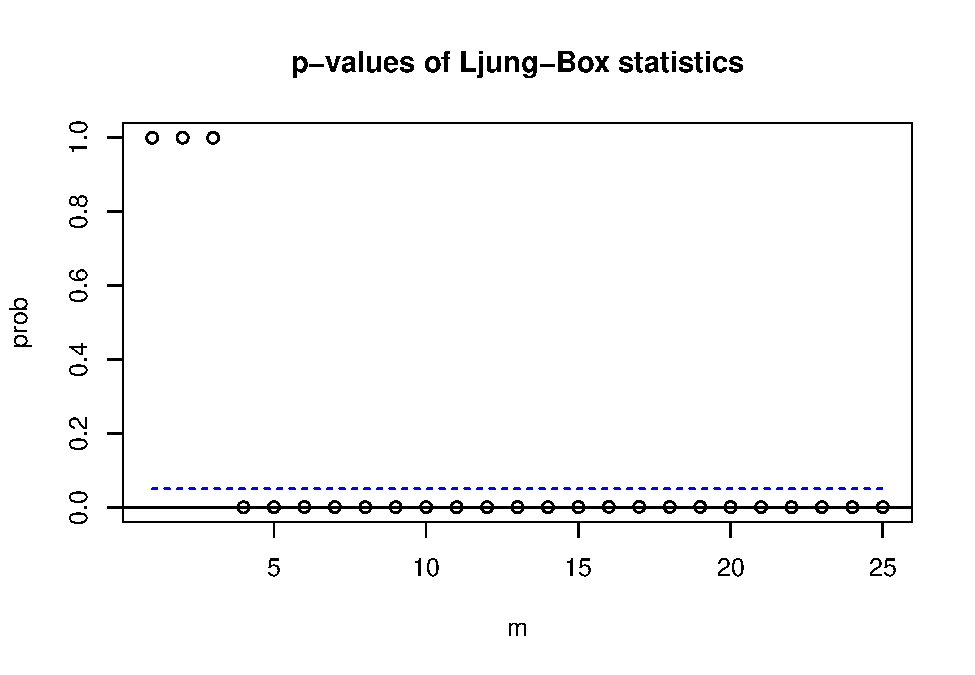
\includegraphics{solution_exercise_6_files/figure-latex/2_f-1.pdf}

\begin{Shaded}
\begin{Highlighting}[]
\KeywordTok{mq}\NormalTok{(var_}\FloatTok{3.}\NormalTok{ref.fit}\OperatorTok{$}\NormalTok{residuals, }\DataTypeTok{lag =} \DecValTok{25}\NormalTok{, }\DataTypeTok{adj =}\NormalTok{ ncoef.var_}\FloatTok{3.}\NormalTok{ref)}
\end{Highlighting}
\end{Shaded}

\begin{verbatim}
## Ljung-Box Statistics:  
##         m       Q(m)     df    p-value
##  [1,]   1.0      18.7    -5.0        1
##  [2,]   2.0      49.7    20.0        1
##  [3,]   3.0      77.4    45.0        0
##  [4,]   4.0     121.7    70.0        0
##  [5,]   5.0     145.3    95.0        0
##  [6,]   6.0     170.9   120.0        0
##  [7,]   7.0     196.3   145.0        0
##  [8,]   8.0     247.3   170.0        0
##  [9,]   9.0     284.0   195.0        0
## [10,]  10.0     320.4   220.0        0
## [11,]  11.0     352.0   245.0        0
## [12,]  12.0     391.7   270.0        0
## [13,]  13.0     415.2   295.0        0
## [14,]  14.0     446.0   320.0        0
## [15,]  15.0     458.6   345.0        0
## [16,]  16.0     481.5   370.0        0
## [17,]  17.0     517.0   395.0        0
## [18,]  18.0     544.1   420.0        0
## [19,]  19.0     573.6   445.0        0
## [20,]  20.0     614.0   470.0        0
## [21,]  21.0     636.7   495.0        0
## [22,]  22.0     669.2   520.0        0
## [23,]  23.0     694.9   545.0        0
## [24,]  24.0     726.9   570.0        0
## [25,]  25.0     756.4   595.0        0
\end{verbatim}

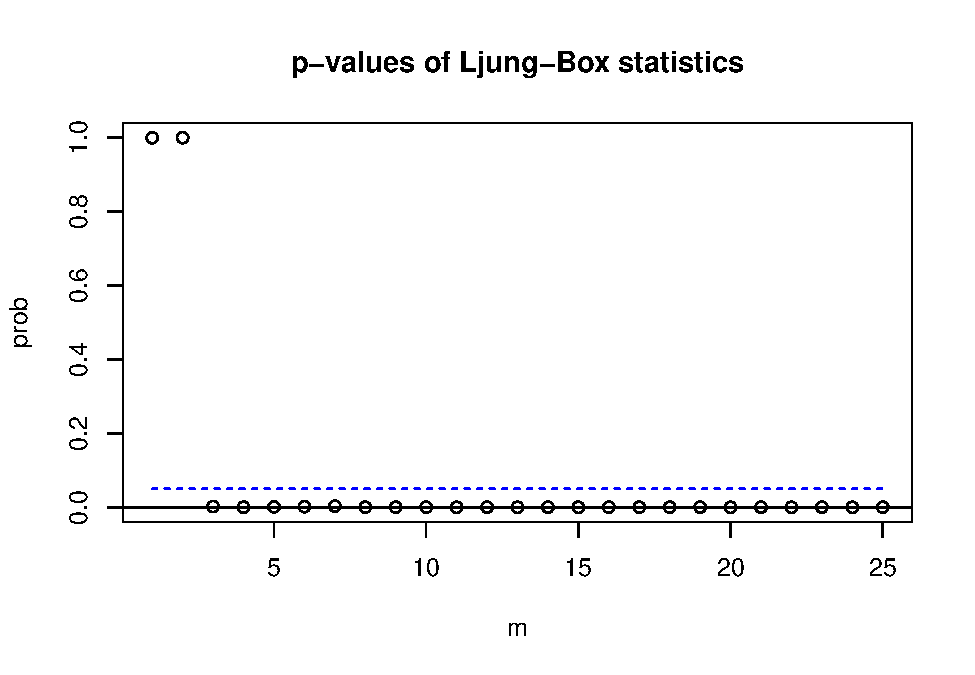
\includegraphics{solution_exercise_6_files/figure-latex/2_f-2.pdf}

\begin{itemize}
  \item[i)] Do the models absorb the dynamics in the data completely?
\end{itemize}

\emph{Solution:}

Ljung-Box test rejects \(H_0\) everywhere, since there are dynamic
patterns in the residuals. A \(\VAR(4)\) did not absorb everything of
the pattern, but we did not expected this after the previous results.

\begin{itemize}
  \item[ii)] Explain the massive differences of the two tests at m = {3, 4}.
\end{itemize}

\emph{Solution:}

The full model uses 75 coefficients, without intercept, while the
redefined model just 30.

\begin{itemize}
  \item[g)] Now estimate a $\VAR(1)$ model (with intercept). How does it compare to the $\VAR(3)$ model in terms of $\MSE$?
\end{itemize}

\emph{Solution:}

\begin{Shaded}
\begin{Highlighting}[]
\NormalTok{var_}\FloatTok{1.}\NormalTok{fit <-}\StringTok{ }\KeywordTok{VAR}\NormalTok{(}\DataTypeTok{x =}\NormalTok{ macdata, }\DataTypeTok{p =} \DecValTok{1}\NormalTok{, }\DataTypeTok{include.mean =} \OtherTok{TRUE}\NormalTok{)}
\end{Highlighting}
\end{Shaded}

\begin{verbatim}
## Constant term: 
## Estimates:  0.0006524376 0.0004706507 0.1048617 -0.04570757 -0.009633996 
## Std.Error:  0.001716609 0.002438123 0.08110986 0.01120102 0.005156064 
## AR coefficient matrix 
## AR( 1 )-matrix 
##          [,1]    [,2]     [,3]    [,4]    [,5]
## [1,]  0.72558  0.0422 0.000393 -0.0253 -0.0755
## [2,] -0.16622  0.3665 0.001002 -0.0369 -0.0489
## [3,]  9.70625 -8.8835 0.985534 -3.9430  2.7900
## [4,] -0.03134  1.7298 0.009042 -0.2355 -0.6760
## [5,] -0.00339  0.1806 0.002089 -0.0590  0.3043
## standard error 
##        [,1]   [,2]     [,3]   [,4]   [,5]
## [1,] 0.0519 0.0825 0.000278 0.0167 0.0316
## [2,] 0.0737 0.1172 0.000395 0.0237 0.0448
## [3,] 2.4510 3.8991 0.013150 0.7876 1.4912
## [4,] 0.3385 0.5385 0.001816 0.1088 0.2059
## [5,] 0.1558 0.2479 0.000836 0.0501 0.0948
##   
## Residuals cov-mtx: 
##               [,1]          [,2]          [,3]          [,4]          [,5]
## [1,]  2.616396e-05  5.011600e-06 -0.0001337874  2.459967e-05 -2.236565e-05
## [2,]  5.011600e-06  5.278030e-05 -0.0004802772  1.887306e-04 -7.099746e-05
## [3,] -1.337874e-04 -4.802772e-04  0.0584128103 -2.844944e-03  1.130147e-03
## [4,]  2.459967e-05  1.887306e-04 -0.0028449444  1.113976e-03 -2.982007e-04
## [5,] -2.236565e-05 -7.099746e-05  0.0011301473 -2.982007e-04  2.360464e-04
##   
## det(SSE) =  3.783152e-18 
## AIC =  -39.86217 
## BIC =  -39.44552 
## HQ  =  -39.6935
\end{verbatim}

\begin{Shaded}
\begin{Highlighting}[]
\KeywordTok{diag}\NormalTok{(var_}\FloatTok{1.}\NormalTok{fit}\OperatorTok{$}\NormalTok{Sigma) }\OperatorTok{/}\StringTok{ }\KeywordTok{diag}\NormalTok{(var_}\FloatTok{3.}\NormalTok{fit}\OperatorTok{$}\NormalTok{Sigma)}
\end{Highlighting}
\end{Shaded}

\begin{verbatim}
## [1] 1.228895 1.118259 1.848220 1.127132 1.079123
\end{verbatim}

\begin{Shaded}
\begin{Highlighting}[]
\KeywordTok{det}\NormalTok{(var_}\FloatTok{1.}\NormalTok{fit}\OperatorTok{$}\NormalTok{Sigma) }\OperatorTok{/}\StringTok{ }\KeywordTok{det}\NormalTok{(var_}\FloatTok{3.}\NormalTok{fit}\OperatorTok{$}\NormalTok{Sigma)}
\end{Highlighting}
\end{Shaded}

\begin{verbatim}
## [1] 3.263859
\end{verbatim}

The \(\VAR(3)\) performs also better then a \(\VAR(1) \ \MSE\)-wise. Not
surprisingly at in-sample, see e.

\begin{itemize}
  \item[h)] Lastly, compute the forecasts’ $\MSE$s (referred to as MSFE) for both models using the command `VARpred`. Please use a forecast horizon h of 10.
\end{itemize}

\emph{Solution:}

\begin{Shaded}
\begin{Highlighting}[]
\NormalTok{var_}\FloatTok{1.}\NormalTok{pred <-}\StringTok{ }\KeywordTok{VARpred}\NormalTok{(}\DataTypeTok{model =}\NormalTok{ var_}\FloatTok{1.}\NormalTok{fit, }\DataTypeTok{h =} \DecValTok{10}\NormalTok{)}
\end{Highlighting}
\end{Shaded}

\begin{verbatim}
## orig  197 
## Forecasts at origin:  197 
##           [,1]     [,2]  [,3]      [,4]       [,5]
##  [1,] 0.008722 0.005923 3.992 0.0080434 -3.574e-03
##  [2,] 0.008867 0.005069 4.029 0.0008851 -1.817e-03
##  [3,] 0.008999 0.004947 4.109 0.0002384 -9.365e-04
##  [4,] 0.009071 0.004941 4.194 0.0002959 -4.877e-04
##  [5,] 0.009122 0.004988 4.280 0.0007365 -1.778e-04
##  [6,] 0.009159 0.005051 4.363 0.0012791  7.813e-05
##  [7,] 0.009189 0.005119 4.444 0.0018445  3.103e-04
##  [8,] 0.009214 0.005188 4.522 0.0024037  5.289e-04
##  [9,] 0.009234 0.005256 4.597 0.0029469  7.375e-04
## [10,] 0.009252 0.005322 4.669 0.0034709  9.373e-04
## Standard Errors of predictions:  
##           [,1]     [,2]   [,3]    [,4]    [,5]
##  [1,] 0.005115 0.007265 0.2417 0.03338 0.01536
##  [2,] 0.006539 0.007630 0.4410 0.03669 0.01626
##  [3,] 0.007179 0.007687 0.6050 0.03675 0.01648
##  [4,] 0.007511 0.007730 0.7332 0.03683 0.01656
##  [5,] 0.007687 0.007760 0.8371 0.03693 0.01661
##  [6,] 0.007783 0.007779 0.9239 0.03704 0.01665
##  [7,] 0.007835 0.007792 0.9982 0.03714 0.01668
##  [8,] 0.007864 0.007802 1.0627 0.03723 0.01672
##  [9,] 0.007880 0.007809 1.1193 0.03732 0.01674
## [10,] 0.007889 0.007816 1.1693 0.03740 0.01677
## Root mean square errors of predictions:  
##           [,1]     [,2]    [,3]    [,4]   [,5]
##  [1,] 0.005192 0.007375  0.2453 0.03388 0.0156
##  [2,] 0.705114 0.403543 63.8382 2.63617 0.9229
##  [3,] 0.513008 0.162239 71.6994 0.36968 0.4636
##  [4,] 0.382002 0.140978 71.6973 0.41900 0.2861
##  [5,] 0.283639 0.117478 69.9009 0.48379 0.2222
##  [6,] 0.210677 0.095129 67.6873 0.48522 0.1960
##  [7,] 0.156631 0.078414 65.4039 0.47118 0.1831
##  [8,] 0.116693 0.067173 63.1158 0.45493 0.1748
##  [9,] 0.087233 0.060026 60.8354 0.43921 0.1682
## [10,] 0.065543 0.055507 58.5704 0.42412 0.1622
\end{verbatim}

\begin{Shaded}
\begin{Highlighting}[]
\NormalTok{var_}\FloatTok{3.}\NormalTok{pred <-}\StringTok{ }\KeywordTok{VARpred}\NormalTok{(}\DataTypeTok{model =}\NormalTok{ var_}\FloatTok{3.}\NormalTok{fit, }\DataTypeTok{h =} \DecValTok{10}\NormalTok{)}
\end{Highlighting}
\end{Shaded}

\begin{verbatim}
## orig  197 
## Forecasts at origin:  197 
##           [,1]     [,2]  [,3]     [,4]       [,5]
##  [1,] 0.007769 0.006092 4.081 0.009667 -2.226e-03
##  [2,] 0.006417 0.005455 4.172 0.004432 -1.661e-03
##  [3,] 0.006934 0.006130 4.266 0.007252 -1.992e-03
##  [4,] 0.007787 0.005867 4.367 0.005236 -6.408e-04
##  [5,] 0.007630 0.005721 4.478 0.005341  1.524e-05
##  [6,] 0.007852 0.005875 4.588 0.006116  2.508e-04
##  [7,] 0.008191 0.005952 4.699 0.006403  8.293e-04
##  [8,] 0.008297 0.005967 4.808 0.007047  1.216e-03
##  [9,] 0.008451 0.006060 4.913 0.007795  1.459e-03
## [10,] 0.008632 0.006130 5.012 0.008321  1.772e-03
## Standard Errors of predictions:  
##           [,1]     [,2]   [,3]    [,4]    [,5]
##  [1,] 0.004614 0.006870 0.1778 0.03144 0.01479
##  [2,] 0.005543 0.007207 0.3471 0.03493 0.01549
##  [3,] 0.005834 0.007515 0.5056 0.03645 0.01581
##  [4,] 0.006262 0.007572 0.6660 0.03675 0.01639
##  [5,] 0.006659 0.007608 0.8131 0.03688 0.01666
##  [6,] 0.006894 0.007663 0.9423 0.03708 0.01676
##  [7,] 0.007083 0.007701 1.0501 0.03725 0.01684
##  [8,] 0.007251 0.007732 1.1386 0.03741 0.01689
##  [9,] 0.007378 0.007761 1.2102 0.03757 0.01692
## [10,] 0.007479 0.007781 1.2681 0.03769 0.01694
## Root mean square errors of predictions:  
##           [,1]     [,2]     [,3]     [,4]    [,5]
##  [1,] 0.004798 0.007144   0.1849  0.03269 0.01538
##  [2,] 2.072861 1.470646 201.1592 10.27156 3.10502
##  [3,] 1.227546 1.435967 248.0941  7.04102 2.13880
##  [4,] 1.536335 0.623325 292.5700  3.13470 2.92281
##  [5,] 1.528387 0.504341 314.8219  2.07860 1.99568
##  [6,] 1.204334 0.616768 321.3266  2.61215 1.26442
##  [7,] 1.095587 0.513635 312.7534  2.39174 1.12425
##  [8,] 1.046496 0.470372 297.0697  2.34716 0.87519
##  [9,] 0.921178 0.447960 276.7477  2.32674 0.63992
## [10,] 0.825714 0.377270 255.6431  1.99677 0.58559
\end{verbatim}

\begin{itemize}
  \item[i)] Does the model superior in f) still prevail at every h?
\end{itemize}

\emph{Solution:}

\begin{Shaded}
\begin{Highlighting}[]
\NormalTok{var_}\FloatTok{1.}\NormalTok{pred}\OperatorTok{$}\NormalTok{rmse }\OperatorTok{/}\StringTok{ }\NormalTok{var_}\FloatTok{3.}\NormalTok{pred}\OperatorTok{$}\NormalTok{rmse}
\end{Highlighting}
\end{Shaded}

\begin{verbatim}
##             [,1]      [,2]      [,3]       [,4]       [,5]
##  [1,] 1.08221998 1.0323561 1.3271960 1.03644347 1.01413021
##  [2,] 0.34016444 0.2743983 0.3173516 0.25664729 0.29722459
##  [3,] 0.41791375 0.1129826 0.2890007 0.05250421 0.21676409
##  [4,] 0.24864505 0.2261703 0.2450605 0.13366564 0.09787525
##  [5,] 0.18558031 0.2329339 0.2220332 0.23274606 0.11131688
##  [6,] 0.17493226 0.1542386 0.2106496 0.18575354 0.15503482
##  [7,] 0.14296532 0.1526650 0.2091231 0.19700271 0.16287921
##  [8,] 0.11150869 0.1428086 0.2124613 0.19382054 0.19977943
##  [9,] 0.09469717 0.1339985 0.2198226 0.18876828 0.26288521
## [10,] 0.07937792 0.1471278 0.2291100 0.21240438 0.27697552
\end{verbatim}

At \(h = 1\), the \(\VAR(3)\) is better. (As \(h = 1\) corresponds to
the in-sample \(\MSE\), this is hardly surprising.) But as \(h \geq 2\),
the sparser \(\VAR(1)\) model fairs much better, because it is less
prone to overfitting which hurts the out-of-sample forecasts.

\begin{itemize}
  \item[ii)] Explain what conceptual difference bewteen $\MSE$ and $\text{MSFE}$ drives the resuls in i). 
\end{itemize}

\emph{Solution:}

\begin{itemize}
  \item MSE: in-sample predicting error
  \begin{itemize}   
    \item Same Data is used for fitting and evaluating of the model. Problem of overfitting could potential araise. 
  \end{itemize}
  \item MSFE: out-of-sample predicting error
  \begin{itemize}   
    \item Different Data is used for fitting and evaluating of the model. So the problem of overfitting is avoided.
  \end{itemize}
\end{itemize}

\begin{itemize}
  \item[iii)] To which values do the forecasts converge to if $h$ goes to $\infty$?
\end{itemize}

\begin{Shaded}
\begin{Highlighting}[]
\CommentTok{# deviations from mean}
\NormalTok{var_}\FloatTok{1.}\NormalTok{pred}\OperatorTok{$}\NormalTok{pred }\OperatorTok{-}\StringTok{ }\KeywordTok{matrix}\NormalTok{(}\DataTypeTok{data =} \KeywordTok{colMeans}\NormalTok{(macdata), }
                         \DataTypeTok{nrow =} \DecValTok{10}\NormalTok{, }\DataTypeTok{ncol =} \DecValTok{5}\NormalTok{, }\DataTypeTok{byrow =} \OtherTok{TRUE}\NormalTok{)}
\end{Highlighting}
\end{Shaded}

\begin{verbatim}
##                [,1]          [,2]      [,3]         [,4]         [,5]
##  [1,] -0.0009308481 -0.0009238241 -2.339300 -0.007716632 -0.009007171
##  [2,] -0.0007856999 -0.0017786759 -2.301837 -0.014874960 -0.007249986
##  [3,] -0.0006532736 -0.0019001751 -2.222785 -0.015521678 -0.006369408
##  [4,] -0.0005813275 -0.0019067256 -2.137505 -0.015464158 -0.005920551
##  [5,] -0.0005311935 -0.0018597422 -2.051676 -0.015023576 -0.005610652
##  [6,] -0.0004936130 -0.0017963123 -1.967893 -0.014481018 -0.005354758
##  [7,] -0.0004637550 -0.0017279406 -1.886945 -0.013915615 -0.005122574
##  [8,] -0.0004391954 -0.0016589988 -1.809068 -0.013356417 -0.004903959
##  [9,] -0.0004184827 -0.0015911497 -1.734286 -0.012813195 -0.004695399
## [10,] -0.0004006619 -0.0015250806 -1.662548 -0.012289175 -0.004495605
\end{verbatim}

\begin{Shaded}
\begin{Highlighting}[]
\NormalTok{var_}\FloatTok{3.}\NormalTok{pred}\OperatorTok{$}\NormalTok{pred }\OperatorTok{-}\StringTok{ }\KeywordTok{matrix}\NormalTok{(}\DataTypeTok{data =} \KeywordTok{colMeans}\NormalTok{(macdata), }
                         \DataTypeTok{nrow =} \DecValTok{10}\NormalTok{, }\DataTypeTok{ncol =} \DecValTok{5}\NormalTok{, }\DataTypeTok{byrow =} \OtherTok{TRUE}\NormalTok{)}
\end{Highlighting}
\end{Shaded}

\begin{verbatim}
##               [,1]          [,2]      [,3]         [,4]         [,5]
##  [1,] -0.001883544 -0.0007555704 -2.250274 -0.006092947 -0.007659215
##  [2,] -0.003236090 -0.0013924001 -2.159637 -0.011327765 -0.007094231
##  [3,] -0.002718484 -0.0007168289 -2.065514 -0.008508153 -0.007425388
##  [4,] -0.001866159 -0.0009807007 -1.964194 -0.010523850 -0.006073741
##  [5,] -0.002022726 -0.0011262015 -1.853396 -0.010418845 -0.005417649
##  [6,] -0.001800495 -0.0009724132 -1.742955 -0.009644073 -0.005182115
##  [7,] -0.001461997 -0.0008955327 -1.632514 -0.009357422 -0.004603569
##  [8,] -0.001355442 -0.0008798122 -1.523163 -0.008713018 -0.004216821
##  [9,] -0.001202226 -0.0007876886 -1.418728 -0.007965395 -0.003974333
## [10,] -0.001020473 -0.0007169872 -1.319314 -0.007439477 -0.003661298
\end{verbatim}

They converge to the means of \(\mathbb{E}(z_t)\) because this process
is stationary and the influence of \(a_t, a_{t-1}, \ldots, a_{0}\)
vanishes as \(h \rightarrow \infty\),

\hypertarget{exercise-3-simplicfication-and-forecasting-exchange-rates}{%
\section{Exercise 3: Simplicfication and Forecasting -- Exchange
Rates}\label{exercise-3-simplicfication-and-forecasting-exchange-rates}}

\begin{itemize}
  \item[a)] Fit a $\VAR(1)$ model to the data regardless of the information criteria.
\end{itemize}

\emph{Solution:}

\begin{Shaded}
\begin{Highlighting}[]
\NormalTok{fx_var1.fit <-}\StringTok{ }\KeywordTok{VAR}\NormalTok{(}\DataTypeTok{x =}\NormalTok{ fx_series, }\DataTypeTok{p =} \DecValTok{1}\NormalTok{, }\DataTypeTok{include.mean =} \OtherTok{TRUE}\NormalTok{)}
\end{Highlighting}
\end{Shaded}

\begin{verbatim}
## Constant term: 
## Estimates:  -5.019648e-06 -2.684985e-06 
## Std.Error:  8.707697e-05 9.152714e-05 
## AR coefficient matrix 
## AR( 1 )-matrix 
##          [,1]    [,2]
## [1,] 0.016600  0.0287
## [2,] 0.000201 -0.0217
## standard error 
##        [,1]   [,2]
## [1,] 0.0147 0.0140
## [2,] 0.0155 0.0147
##   
## Residuals cov-mtx: 
##               [,1]          [,2]
## [1,]  3.804083e-05 -1.128310e-05
## [2,] -1.128310e-05  4.202843e-05
##   
## det(SSE) =  1.471488e-09 
## AIC =  -20.3354 
## BIC =  -20.3302 
## HQ  =  -20.33358
\end{verbatim}

\begin{itemize}
  \item[b)] Now fit the refined model based on your VAR(1) setting the threshold to 1.96. How many coefficients have been set to zero?
\end{itemize}

\emph{Solution:}

\begin{Shaded}
\begin{Highlighting}[]
\NormalTok{fx_var1.ref.fit <-}\StringTok{ }\KeywordTok{refVAR}\NormalTok{(}\DataTypeTok{model =}\NormalTok{ fx_var1.fit, }\DataTypeTok{thres =} \FloatTok{1.96}\NormalTok{)}
\end{Highlighting}
\end{Shaded}

\begin{verbatim}
## Constant term: 
## Estimates:  0 0 
## Std.Error:  0 0 
## AR coefficient matrix 
## AR( 1 )-matrix 
##      [,1] [,2]
## [1,]    0    0
## [2,]    0    0
## standard error 
##      [,1] [,2]
## [1,]    0    0
## [2,]    0    0
##   
## Residuals cov-mtx: 
##               resi          resi
## resi  3.807533e-05 -1.130523e-05
## resi -1.130523e-05  4.204841e-05
##   
## det(SSE) =  1.473199e-09 
## AIC =  -20.33583 
## BIC =  -20.33583 
## HQ  =  -20.33583
\end{verbatim}

The Number of coefficients which are not set to zero are 0. The means of
the series: \ensuremath{-6.0948723\times 10^{-6}},
\ensuremath{-4.3991025\times 10^{-6}} very close to zero.

\begin{itemize}
  \item[c)] Compare the MSEs of the ‘ordinary’ model and the refined model.
\end{itemize}

\emph{Solution:}

\begin{Shaded}
\begin{Highlighting}[]
\KeywordTok{diag}\NormalTok{(fx_var1.fit}\OperatorTok{$}\NormalTok{Sigma) }\OperatorTok{/}\StringTok{ }\KeywordTok{diag}\NormalTok{(fx_var1.ref.fit}\OperatorTok{$}\NormalTok{Sigma)}
\end{Highlighting}
\end{Shaded}

\begin{verbatim}
##      resi      resi 
## 0.9990940 0.9995248
\end{verbatim}

\begin{Shaded}
\begin{Highlighting}[]
\KeywordTok{det}\NormalTok{(fx_var1.fit}\OperatorTok{$}\NormalTok{Sigma) }\OperatorTok{/}\StringTok{ }\KeywordTok{det}\NormalTok{(fx_var1.ref.fit}\OperatorTok{$}\NormalTok{Sigma)}
\end{Highlighting}
\end{Shaded}

\begin{verbatim}
## [1] 0.9988387
\end{verbatim}

Virtually the same. though the \(\VAR(1)\) explains tiny bits of the
variation.

\begin{itemize}
  \item[d)] Thirdly, estimate a $\VAR(0)$ with intercept by regression. Compare its MSFE with the forecast errors of the ‘ordinary’ $\VAR(1)$ model regarding a forecast horizon $h = 10$.
\end{itemize}

\emph{Solution:}

\begin{Shaded}
\begin{Highlighting}[]
\NormalTok{fx_var0.predictions <-}\StringTok{ }\KeywordTok{colMeans}\NormalTok{(fx_series) }
\NormalTok{fx_var0.msfe <-}\StringTok{ }\KeywordTok{colMeans}\NormalTok{( (}\KeywordTok{cbind}\NormalTok{(fx_series[,}\DecValTok{1}\NormalTok{] }\OperatorTok{-}\StringTok{ }\NormalTok{fx_var0.predictions[}\DecValTok{1}\NormalTok{], fx_series[,}\DecValTok{2}\NormalTok{] }\OperatorTok{-}\StringTok{ }\NormalTok{fx_var0.predictions[}\DecValTok{2}\NormalTok{]))}\OperatorTok{^}\DecValTok{2}\NormalTok{ )}
\NormalTok{fx_var0.rmse <-}\StringTok{ }\KeywordTok{sqrt}\NormalTok{(fx_var0.msfe)}
\NormalTok{fx_var1.pred <-}\StringTok{ }\KeywordTok{VARpred}\NormalTok{(}\DataTypeTok{model =}\NormalTok{ fx_var1.fit, }\DataTypeTok{h =} \DecValTok{10}\NormalTok{)}
\end{Highlighting}
\end{Shaded}

\begin{verbatim}
## orig  5021 
## Forecasts at origin:  5021 
##            lr.Eu      lr.Ja
##  [1,] -1.563e-04  1.240e-04
##  [2,] -4.051e-06 -5.411e-06
##  [3,] -5.242e-06 -2.568e-06
##  [4,] -5.181e-06 -2.630e-06
##  [5,] -5.181e-06 -2.629e-06
##  [6,] -5.181e-06 -2.629e-06
##  [7,] -5.181e-06 -2.629e-06
##  [8,] -5.181e-06 -2.629e-06
##  [9,] -5.181e-06 -2.629e-06
## [10,] -5.181e-06 -2.629e-06
## Standard Errors of predictions:  
##           [,1]     [,2]
##  [1,] 0.006168 0.006483
##  [2,] 0.006171 0.006484
##  [3,] 0.006171 0.006484
##  [4,] 0.006171 0.006484
##  [5,] 0.006171 0.006484
##  [6,] 0.006171 0.006484
##  [7,] 0.006171 0.006484
##  [8,] 0.006171 0.006484
##  [9,] 0.006171 0.006484
## [10,] 0.006171 0.006484
## Root mean square errors of predictions:  
##           [,1]     [,2]
##  [1,] 0.006170 0.006485
##  [2,] 0.006209 0.006506
##  [3,] 0.006171 0.006484
##  [4,] 0.006171 0.006484
##  [5,] 0.006171 0.006484
##  [6,] 0.006171 0.006484
##  [7,] 0.006171 0.006484
##  [8,] 0.006171 0.006484
##  [9,] 0.006171 0.006484
## [10,] 0.006171 0.006484
\end{verbatim}

The ratio of the forecast errors are:

\begin{Shaded}
\begin{Highlighting}[]
\NormalTok{fx_var1.pred}\OperatorTok{$}\NormalTok{rmse }\OperatorTok{/}\StringTok{ }\KeywordTok{matrix}\NormalTok{(}\DataTypeTok{data =}\NormalTok{ fx_var0.rmse, }\DataTypeTok{nrow =} \DecValTok{10}\NormalTok{, }\DataTypeTok{byrow =} \OtherTok{TRUE}\NormalTok{, }\DataTypeTok{ncol =} \DecValTok{2}\NormalTok{)}
\end{Highlighting}
\end{Shaded}

\begin{verbatim}
##            [,1]      [,2]
##  [1,] 0.9998946 0.9999708
##  [2,] 1.0063092 1.0031989
##  [3,] 1.0000495 0.9999113
##  [4,] 1.0000486 0.9999097
##  [5,] 1.0000486 0.9999097
##  [6,] 1.0000486 0.9999097
##  [7,] 1.0000486 0.9999097
##  [8,] 1.0000486 0.9999097
##  [9,] 1.0000486 0.9999097
## [10,] 1.0000486 0.9999097
\end{verbatim}

\(\VAR(0)\) with intercept:

\begin{align*}
  z_t & = \phi_0 + a_t\\
  \Rightarrow \hat{\phi_0} & = \argmin_{\phi_0} \sum_{t = 1}^{T} \left(z_t - \phi_0 \right)^{'} \left(z_t - \phi_0 \right)\\
  \Rightarrow \hat{\phi}_0 & = \dfrac{1}{T} \sum_{t = 1}^{T} z_t \rightarrow \mathbb{E} (z_t)\\
  \Rightarrow \hat{z}_{t,t+h} &= = \bar{z_t} = \hat{\phi}_0
\end{align*}

The \(\VAR(1)\) does slightly better at \(h = \left\{ 1,2,3 \right\}\)
but then the forecast errors align because the \(\VAR(1)\) forecast has
returned to the mean.

\begin{itemize}
  \item[e)] How do your results in d) align with the insights you gained in exercise 2h)?
\end{itemize}

\emph{Solution:}

The \(\VAR(1)\) might be overspecified, but this did not lead to
considerable overfitting. Primarily this is due to the small number of
coefficients and the large sample size
\(\left( \dfrac{\# \text{coefs}}{\# \text{data points}} \; \; \text{remains small}\right)\)

\begin{itemize}
  \item[f)]  What can you do to reproduce the findings from 2h) in this setting?
\end{itemize}

\emph{Solution:}

\begin{Shaded}
\begin{Highlighting}[]
\NormalTok{var25.fit <-}\StringTok{ }\KeywordTok{VAR}\NormalTok{(}\DataTypeTok{x =}\NormalTok{ fx_series[}\DecValTok{1}\OperatorTok{:}\DecValTok{500}\NormalTok{,], }\DataTypeTok{p =} \DecValTok{25}\NormalTok{, }\DataTypeTok{include.mean =} \OtherTok{TRUE}\NormalTok{, }\DataTypeTok{output =} \OtherTok{FALSE}\NormalTok{)}
\NormalTok{var25.pred <-}\StringTok{ }\KeywordTok{VARpred}\NormalTok{(}\DataTypeTok{model =}\NormalTok{ var25.fit, }\DataTypeTok{h =} \DecValTok{10}\NormalTok{, }\DataTypeTok{output =} \OtherTok{FALSE}\NormalTok{)}
\end{Highlighting}
\end{Shaded}

\begin{verbatim}
## orig  500
\end{verbatim}

\begin{Shaded}
\begin{Highlighting}[]
\NormalTok{var25.pred}\OperatorTok{$}\NormalTok{rmse }\OperatorTok{/}\StringTok{ }\NormalTok{fx_var1.pred}\OperatorTok{$}\NormalTok{rmse}
\end{Highlighting}
\end{Shaded}

\begin{verbatim}
##           [,1]     [,2]
##  [1,] 1.065278 1.096485
##  [2,] 5.759076 1.623631
##  [3,] 2.179696 3.392377
##  [4,] 2.241620 2.135705
##  [5,] 5.304804 3.650994
##  [6,] 4.145933 4.549648
##  [7,] 4.886221 3.987958
##  [8,] 3.059212 3.946744
##  [9,] 3.646427 7.089310
## [10,] 2.589909 2.147618
\end{verbatim}

Note the chaotic (non-)structure in the MSFE! Usually it should rise
with \(h\). Reduce the number of observations massively and raise the
number of coefficients distinctly. This will produce overfitting.

The forecasts will converge to the mean quickly (faster than in 2)h) ),
since there is barly any autocorrelation so the innovations' effects
vanish almost immediately. And trivially, the MSFE (out-of-sample) will
be similar to the MSE (in-sample), because there is effectively no model
to be found except the global mean.

\hypertarget{exercise-4-forecast-errors}{%
\section{Exercise 4: Forecast Errors}\label{exercise-4-forecast-errors}}

Show that Equation (5.1) in the lecture slides implies that
\[ \mathbb{E} \left[ \hat{z}_{T,\ T + h}^{(i)} - z_{T+h} \right]^2 \geq \mathbb{E} \left[ \hat{z}_{T}^{(i)}  (h)- z_{T+h} \right]^2 \text{,}\]

where \(\hat{z}_{T, T+h}^{(i)}\) and \(z_T^{(i)} (h)\) denote the
\(i\)-th components of the respective forecasts \((i = 1, \dots ,K)\)
for the observation \(z_{T+h}\). This means that the optimal univariate
forecasts are simply the components of the optimal \emph{multivariate}
forecast \(z_T (h)\).

\emph{Solution:}

\begin{itemize}
  \item $\hat{z}_{T, T+h}^{(i)}$: $h$-steps ahead forecast of variable $i$ at time $T$ 
  \item $\hat{z}_{T}^{(i)} (h)$: optimal $h$-steps ahead forecast of variable $i$ at time $T$
\end{itemize}

\underline{Multivariate:} Equation 5.1

\begin{align*}
  \left| \text{MSE} \left( \hat{z}_{T, T+h} \right) \right| & \geq \left| \text{MSE} \left( \hat{z}_{T} (h) \right) \right| \\
  \left| \text{MSE} \left( \hat{z}_{T, T+h} \right) - \text{MSE} \left( \hat{z}_{T} (h) \right) \right| & \geq 0 \\
  & \text{$\rightarrow$ a p.s.d. matrix! }
\end{align*}

From slide (5-5) we know:

\begin{align*}
  \mathbb{E} \left[ \left( z_T (h) - \hat{z}_{T, T+h}\right) \left( z_T (h) - \hat{z}_{T, T+h}\right)^{'} \right] & \geq 0 =: A\\
\end{align*}

For any p.s.d. matrix \(A\) and vector \(w\) it holds that

\begin{align*}
  w^{'} A w & \geq 0 \\
  \\
  \text{Define} \ w & = \begin{pmatrix} 0 \\ \vdots \\ 0 \\ 1 \\ 0 \vdots \\ 0 \end{pmatrix} \leftarrow \ \text{only 1 at indes} i \text{!}
\end{align*}

\begin{itemize}
  \item $w^{'} A$ is $0$ everywhere except at row $i$ and $Aw$ sets every column except $i$ to zero. 
  \item $w^{'}A w$ is only $\neq 0$ at the $i^{th}$ element on the main diagonal!
\end{itemize}

That means:

\begin{align*}
  w^{'} A w & = \mathbb{E} \left[ \left( z_T^{(i)} (h) - z_{T, T+h}^{(i)} (h) \right)^2 \right]\\
  & \geq 0 \ \text{(p.s.d)}\\
  & \text{which corresponds to} \ \; \text{MSE} \left(z_{T, T+h}^{(i)} \right) - \text{MSE} \left(z_{T}^{(i)} \right)\\
  & = \mathbb{E} \left[ \left( \hat{z}_T^{(i)} (h) - z_{T, T+h}^{(i)} (h) \right)^2 \right] - \mathbb{E} \left[ \left( z_T^{(i)} (h) - z_{T, T+h}^{(i)} (h) \right)^2 \right] \\
  & \geq 0
\end{align*}

\end{document}
